%%%%%%%%%%%%%%%%%%%%%%%%%%%%%%%%%%%%%%%%%%%%%%%%%%%%%%%%%%%%%%%%%%%%%% 
%%%%%%%%%%%%%%%%%%%%%%%%%%%%%%%%%%%%%%%%%%%%%%%%%%%%%%%%%%%%%%%%%%%%%% 
\section{Multigrid}
\frame{\tableofcontents[currentsection,hideothersubsections]}

%%%%%%%%%%%%%%%%%%%%%%%%%%%%%%%%%%%%%%%%%%%%%%%%%%%%%%%%%%%%%%%%%%%%%%
\begin{frame}
  \frametitle{Solving the discrete problems}
  \begin{itemize}
  \item Iterative solvers usually slow down when meshes get finer
    \begin{itemize}
    \item $\mathcal O(h^{-p})$ steps for differential operator of order $p$
    \item Number of steps multiplied by 4 each refinement
    \end{itemize}
  \item Krylov space solvers accelerate somewhat
    \begin{itemize}
    \item Conjugate gradient method or GMRES
    \item $\mathcal O(h^{-p/2})$ steps for differential operator of order $p$
    \item Number of steps still doubles with each refinement
    \end{itemize}
  \item ``Preconditioning'' needed for optimality
    \begin{gather*}
      Ax=b \qquad \Rightarrow \qquad B^{-1}Ax = B^{-1}b.
    \end{gather*}
  \end{itemize}
\end{frame}

%%%%%%%%%%%%%%%%%%%%%%%%%%%%%%%%%%%%%%%%%%%%%%%%%%%%%%%%%%%%%%%%%%%%%%
\begin{frame}
  \frametitle{Goal of preconditioning}
  \begin{block}{Optimal complexity}
    A solver has optimal complexity if a system with $n$ variables can
    be solved with $\mathcal O(n)$ operations.
  \end{block}
  \begin{itemize}
  \item Number of iterations independent of mesh size
  \item Preconditioner can be evaluated in $\mathcal O(n)$ operations.
  \end{itemize}
\end{frame}

%%%%%%%%%%%%%%%%%%%%%%%%%%%%%%%%%%%%%%%%%%%%%%%%%%%%%%%%%%%%%%%%%%%%%%
\begin{frame}
  \frametitle{Examples for preconditioners}
  \begin{gather*}
    B^{-1}Ax = B^{-1}b.
  \end{gather*}
  \begin{itemize}
  \item $B=I$: evaluation for free, but increasing number of steps
  \item $B=A$: convergence in one step, but evaluation expensive
    \pause
  \item Multigrid methods: optimal
    \begin{enumerate}
    \item Apply one or few steps of a cheap iteration (smoother) on given level
    \item Project residual to next coarser level
    \item Apply the same method on the coarser level
    \item Improve fine level result by coarse grid correction
    \item Apply one or few smoothing steps on given level
    \end{enumerate}
  \end{itemize}
\end{frame}

\begin{frame}
  \frametitle{Multigrid ingredients}
  \begin{itemize}
  \item Smoother
    \begin{itemize}
    \item (block-)Jacobi, (block-)Gauß-Seidel
    \item overlapping Schwarz methods
    \end{itemize}
  \item Grid transfer
    \begin{itemize}
    \item embedding from coarse to fine
    \item its $\ell_2$-adjoint from fine to coarse
    \end{itemize}
  \item a coarse grid solver
  \end{itemize}
\end{frame}

\begin{frame}
  \frametitle{The V-cycle}
  \begin{columns}
    \begin{column}{.5\textwidth}
    \includegraphics[width=\textwidth]{graph/v-cycle}      
    \end{column}
    \begin{column}{.5\textwidth}
      Recursion on level $\ell$
      \begin{itemize}
      \item 1 smoothing step
      \item Call V-cycle on level $\ell-1$
      \item 1 smoothing step
      \end{itemize}
      Solve on level 0
    \end{column}
  \end{columns}
  \begin{center}
  \end{center}
\end{frame}

\begin{frame}
  \frametitle{The W-cycle}
  \begin{columns}
    \begin{column}{.5\textwidth}
    \includegraphics[width=\textwidth]{graph/w-cycle}
    \end{column}
    \begin{column}{.5\textwidth}
      Recursion on level $\ell$
      \begin{itemize}
      \item 1 smoothing step
      \item Call W-cycle on level $\ell-1$
      \item Call W-cycle on level $\ell-1$
      \item 1 smoothing step
      \end{itemize}
      Solve on level 0
    \end{column}
  \end{columns}
  \begin{center}
  \end{center}
\end{frame}

\begin{frame}
  \frametitle{The F-cycle}
  \begin{columns}
    \begin{column}{.5\textwidth}
    \includegraphics[width=\textwidth]{graph/f-cycle}
    \end{column}
    \begin{column}{.5\textwidth}
      Recursion on level $\ell$
      \begin{itemize}
      \item 1 smoothing step
      \item Call F-cycle on level $\ell-1$
      \item Call V-cycle on level $\ell-1$
      \item 1 smoothing step
      \end{itemize}
      Solve on level 0
    \end{column}
  \end{columns}
  \begin{center}
  \end{center}
\end{frame}


\begin{frame}
  \frametitle{The variable V-cycle}
  \begin{columns}
    \begin{column}{.5\textwidth}
    \includegraphics[width=\textwidth]{graph/vv-cycle}      
    \end{column}
    \begin{column}{.5\textwidth}
      Recursion on level $\ell$
      \begin{itemize}
      \item $2^{L-\ell}$ smoothing steps
      \item Variable V-cycle on level $\ell-1$
      \item $2^{L-\ell}$ smoothing steps
      \end{itemize}
      Solve on level 0
    \end{column}
  \end{columns}
  \begin{center}
  \end{center}
\end{frame}

%%% Local Variables: 
%%% mode: latex
%%% TeX-master: "slides"
%%% End: 


%%%%%%%%%%%%%%%%%%%%%%%%%%%%%%%%%%%%%%%%%%%%%%%%%%%%%%%%%%%%%%%%%%%%%%
\begin{frame}
  \frametitle{Tutorial step 16}
  {\footnotesize{\url{http://www.dealii.org/\dealrelease/doxygen/deal.II/step_8.html}}}
  \begin{itemize}
  \item Multigrid structures
  \end{itemize}
\end{frame}

%%%%%%%%%%%%%%%%%%%%%%%%%%%%%%%%%%%%%%%%%%%%%%%%%%%%%%%%%%%%%%%%%%%%%%
\subsection{Multigrid background}
\begin{frame}
  \frametitle{Components of multigrid}
  \begin{itemize}
  \item Grid transfer between meshes: \lstinline!MGTransferPrebuilt!
  \item Level matrices: \lstinline!mg::Matrix!
  \item Smoothers:  \lstinline!mg::SmootherRelaxation!
  \item Coarse grid solver  \lstinline!MGCoarseGridHouseholder!
  \end{itemize}
\end{frame}

%%%%%%%%%%%%%%%%%%%%%%%%%%%%%%%%%%%%%%%%%%%%%%%%%%%%%%%%%%%%%%%%%%%%%%
\begin{frame}
  \frametitle{Multigrid and hanging nodes}
  \begin{center}
    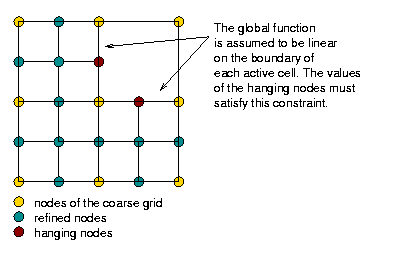
\includegraphics[height=.5\textheight]{graph/hanging_nodes}    
  \end{center}
  \begin{itemize}
  \item Edges with hanging nodes belong to the coarse level
  \item Smoothing only on the fine level
    \begin{itemize}
    \item Zero boundary condition on the edge
    \end{itemize}
  \end{itemize}
\end{frame}

%%%%%%%%%%%%%%%%%%%%%%%%%%%%%%%%%%%%%%%%%%%%%%%%%%%%%%%%%%%%%%%%%%%%%%
\begin{frame}
  \frametitle{Matrices for multigrid}
  \begin{itemize}
  \item Build level matrices with eliminated refinement edge
    \begin{itemize}
    \item Coupling from interior to refinement edge eliminated
    \end{itemize}
  \item Two additional matrices needed for lost couplings
    \begin{itemize}
    \item Needed for computing the whole residual
    \end{itemize}
  \item[$\Rightarrow$] 3 sets of level matrices
  \item Multilevel description of hanging nodes needed
  \end{itemize}
\end{frame}

%%%%%%%%%%%%%%%%%%%%%%%%%%%%%%%%%%%%%%%%%%%%%%%%%%%%%%%%%%%%%%%%%%%%%%
\subsection{Member data in the application class}
\begin{frame}
  \frametitle{Member objects}
  \begin{block}{}
    \lstinputlisting{tutcode/step16-1.cc}
  \end{block}
\end{frame}

%%%%%%%%%%%%%%%%%%%%%%%%%%%%%%%%%%%%%%%%%%%%%%%%%%%%%%%%%%%%%%%%%%%%%%
\subsection{Setting up multilevel data}
\begin{frame}
  \begin{block}{Multilevel setup I}
    \lstinputlisting[basicstyle=\footnotesize]{tutcode/step16-2.cc}
  \end{block}
\end{frame}

\begin{frame}
  \begin{block}{Multilevel setup II}
    \lstinputlisting[basicstyle=\footnotesize]{tutcode/step16-2a.cc}
  \end{block}
\end{frame}

%%%%%%%%%%%%%%%%%%%%%%%%%%%%%%%%%%%%%%%%%%%%%%%%%%%%%%%%%%%%%%%%%%%%%%
%%%%%%%%%%%%%%%%%%%%%%%%%%%%%%%%%%%%%%%%%%%%%%%%%%%%%%%%%%%%%%%%%%%%%%
\subsection{Generic loops}

%%%%%%%%%%%%%%%%%%%%%%%%%%%%%%%%%%%%%%%%%%%%%%%%%%%%%%%%%%%%%%%%%%%%%%
\begin{frame}
  \frametitle{Generic loops through MeshWorker}
  \begin{itemize}
  \item Goal: see loops from an abstract point of view:
      \begin{block}{Generic linear, stationary program}
    \lstinputlisting{assembly2.pseudocode}
  \end{block}  
  \item Application program only implements the local operators
    \item No handling of degrees of freedom or target objects needed
  \end{itemize}
\end{frame}

%%%%%%%%%%%%%%%%%%%%%%%%%%%%%%%%%%%%%%%%%%%%%%%%%%%%%%%%%%%%%%%%%%%%%%
\begin{frame}
  \frametitle{Arguments to local integrator}
  \begin{itemize}
  \item\texttt{MeshWorker::DoFInfo}
    \begin{itemize}
    \item Information on the current cell and its degrees of freedom
    \item Return values in base class \texttt{LocalResults}
    \end{itemize}
  \item\texttt{MeshWorker::IntegrationInfo}
    \begin{itemize}
    \item \texttt{FEValues}
    \item Optional function values in quadrature points
    \end{itemize}
  \end{itemize}
\end{frame}

%%%%%%%%%%%%%%%%%%%%%%%%%%%%%%%%%%%%%%%%%%%%%%%%%%%%%%%%%%%%%%%%%%%%%%
\subsection{Cell matrices}
\begin{frame}
  \frametitle{Class for local integration I}
  \begin{block}{}
    \lstinputlisting[basicstyle=\footnotesize]{tutcode/step16-3.cc}
  \end{block}
\end{frame}

%%%%%%%%%%%%%%%%%%%%%%%%%%%%%%%%%%%%%%%%%%%%%%%%%%%%%%%%%%%%%%%%%%%%%%
\begin{frame}
  \frametitle{Class for local integration II}
  \begin{block}{}
    \lstinputlisting[basicstyle=\footnotesize]{tutcode/step16-3a.cc}
  \end{block}
\end{frame}

%%%%%%%%%%%%%%%%%%%%%%%%%%%%%%%%%%%%%%%%%%%%%%%%%%%%%%%%%%%%%%%%%%%%%%
\begin{frame}
  \frametitle{Setting up the loop I: IterationInfo}
  \begin{itemize}
  \item Handle \texttt{FEValues} objects
  \end{itemize}
  \begin{block}{}
    \lstinputlisting[basicstyle=\small]{tutcode/step16-3b.cc}
  \end{block}
\end{frame}

%%%%%%%%%%%%%%%%%%%%%%%%%%%%%%%%%%%%%%%%%%%%%%%%%%%%%%%%%%%%%%%%%%%%%%
% \begin{frame}
%   \frametitle{Setting up the loop II: Assembler}
%   \begin{block}{}\footnotesize
%     \lstinputlisting{tutcode/step39-6a.cc}
%   \end{block}  
%   \only<1>{\begin{block}{}\footnotesize
%       \lstinputlisting{tutcode/step39-6b.cc}
%     \end{block}}  
%   \only<2->{\begin{block}{}\footnotesize
%       \lstinputlisting{tutcode/step39-6c.cc}
%     \end{block}
%   \begin{block}{}\footnotesize
%     \lstinputlisting{tutcode/step39-6d.cc}
%   \end{block}}
% \end{frame}

%%%%%%%%%%%%%%%%%%%%%%%%%%%%%%%%%%%%%%%%%%%%%%%%%%%%%%%%%%%%%%%%%%%%%%
\begin{frame}
  \frametitle{Setting up the loop III: run!}
  \begin{block}{}\small
    \lstinputlisting{tutcode/step39-7.cc}
  \end{block}
  \pause
  \begin{block}{Multigrid}\small
    \lstinputlisting{tutcode/step39-7b.cc}
  \end{block}
\end{frame}
%%%%%%%%%%%%%%%%%%%%%%%%%%%%%%%%%%%%%%%%%%%%%%%%%%%%%%%%%%%%%%%%%%%%%%
\subsection{Multilevel objects in \lstinline!solve()!}
\begin{frame}
  \frametitle{Transfer operators}
  \begin{block}{}
    \lstinputlisting{tutcode/step16-4.cc}
  \end{block}  
\end{frame}

\begin{frame}
  \frametitle{Coarse grid solver}
  \begin{block}{}
    \lstinputlisting{tutcode/step16-5.cc}
  \end{block}  
\end{frame}

\begin{frame}
  \frametitle{Smoother}
  \begin{block}{}
    \lstinputlisting{tutcode/step16-6.cc}
  \end{block}  
\end{frame}

\begin{frame}
  \frametitle{The \lstinline!Multigrid! object}
  \begin{block}{}
    \lstinputlisting{tutcode/step16-7.cc}
  \end{block}  
\end{frame}

\begin{frame}
  \frametitle{The preconditioner}
  \begin{block}{}
    \lstinputlisting{tutcode/step16-8.cc}
  \end{block}  
\end{frame}

%%%%%%%%%%%%%%%%%%%%%%%%%%%%%%%%%%%%%%%%%%%%%%%%%%%%%%%%%%%%%%%%%%%%%%
\subsection{Problems}
\begin{frame}
  \frametitle{Problems}
  \begin{enumerate}
  \item Compare the results with different cycles
    \begin{itemize}
    \item V-cycle
    \item variable V-cycle
    \item W-cycle
    \item F-cycle
    \end{itemize}
  \item Change the number of smoothing steps
  \item Solve Helmholtz equation instead of Poisson
  \item Add advection in $x$-direction
    \begin{itemize}
    \item Beware of a trick that is used for the interface matrices!
    \end{itemize}
  \end{enumerate}
\end{frame}


%%% Local Variables: 
%%% mode: latex
%%% TeX-master: "slides"
%%% End: 
